\makeatletter
\newenvironment{breakablealgorithm}
  {% \begin{breakablealgorithm}
   \begin{center}
     \refstepcounter{algorithm}% New algorithm
     \hrule height.8pt depth0pt \kern2pt% \@fs@pre for \@fs@ruled
     \renewcommand{\caption}[2][\relax]{% Make a new \caption
       {\raggedright\textbf{\ALG@name~\thealgorithm} ##2\par}%
       \ifx\relax##1\relax % #1 is \relax
         \addcontentsline{loa}{algorithm}{\protect\numberline{\thealgorithm}##2}%
       \else % #1 is not \relax
         \addcontentsline{loa}{algorithm}{\protect\numberline{\thealgorithm}##1}%
       \fi
       \kern2pt\hrule\kern2pt
     }
  }{% \end{breakablealgorithm}
     \kern2pt\hrule\relax% \@fs@post for \@fs@ruled
   \end{center}
  }
\makeatother
\chapter{DDPG Shock Buffer}\label{chapter:ShockBuffer}
In this chapter we analyze some of the problems behind DDPGFunctions described in Chapter \ref{chapter:DDPGFuncs}. We then discuss the reasons why this could happen and ways to mitigate the problems. Afterwards, we present our 2nd version of our DDPG algorithm - DDPG Shock Buffer and explain why in this algorithm, some of the problems in DDPGFunctions get alleviated. We finally explore some hyper parameter constructs with respect to DDPG Shock Buffer and how they impact the simulations.

\section{DDPG Functions - Problems}

We noticed that while DDPG functions provided good results (we discuss them in detail in chapter \ref{chapter:Results}), sometimes we noticed the gradients explode in certain configurations. 

\begin{figure}[htpb]
\centering
  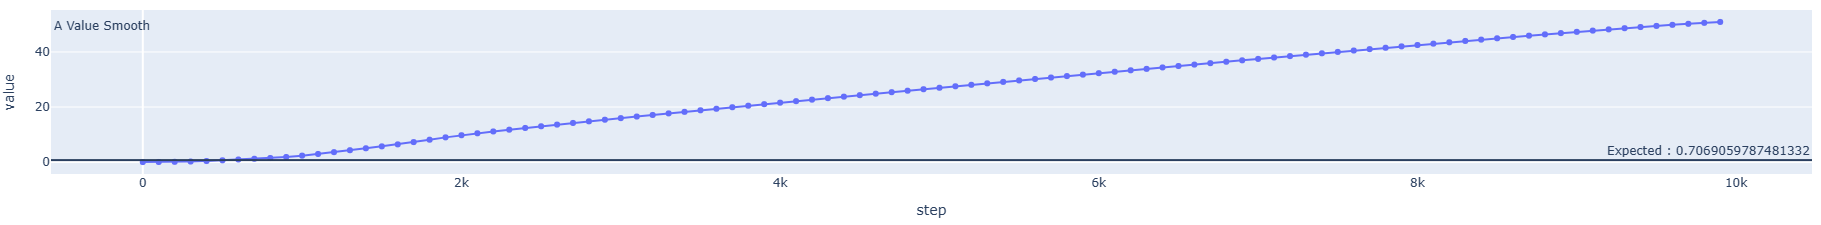
\includegraphics[width=1\textwidth,height=4cm]{figures/DDPGExplod.png}
  \caption[A value Exploding Simulations -DDPG Functions]{A-value ($a^\phi$) during training } \label{fig:expa}
\end{figure}
\begin{figure}[htpb]
\centering
  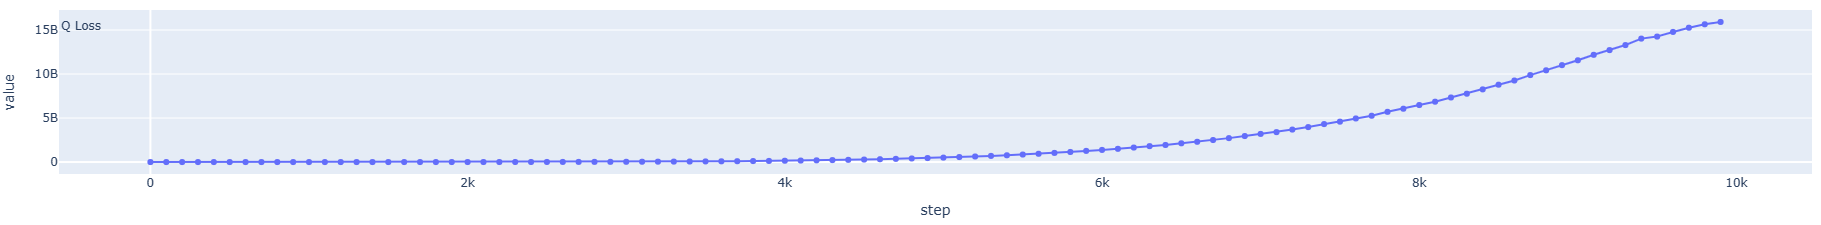
\includegraphics[width=1\textwidth,height=4cm]{figures/DDPGExplodQLoss.png}
  \caption[Q loss Exploding Simulations -DDPG Functions]{Approximate MSBE or "Q-loss" (see (\ref{equation:Eqln}))    during training } \label{fig:expqloss}
\end{figure}

    In Figures \ref{fig:expa} and  \ref{fig:expqloss}, we can see that both MSBE and a-value explode after around 800 training steps.  We saw a non trivial number of experiments (37/1404) , around 2.6\% where the gradients exploded while testing on different market parameters. In addition, we observed that for around 2.5\% of experiments the relative error between the learned portfolio allocation and the optimal allocation was more than 100\%. 


Further, we noticed that in many experiments, the variance of the learned allocation was very high during training.

\begin{figure}[htpb]
  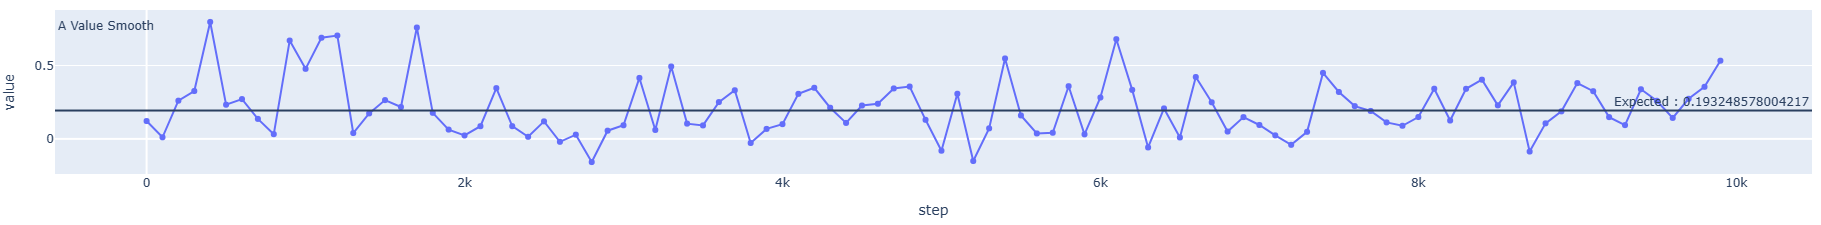
\includegraphics[width=1.0\textwidth,height=4cm]{figures/variance_ddpg.png}
  \caption[Variance of A value]{Example of high variance of $a^\phi$ during training} \label{fig:variance-ddpg}
\end{figure}

In addition to both these issues, we also wanted to explore and obtain more accurate approximation $a^\phi$ for the optimal portfolio $\pi^*$ .

\section{Key Idea}

To understand what could be a key area of improvement let us restate the Bellman optimality equation defined in Chapter \ref{chapter:PO_Problem}

\begin{equation} \label{eq:BMO1}
\begin{array}
 Q Q^*(s,a) = \underset{s' \sim P}{{\mathbb E}}\left[r(s,a,s') + (1-d) \max_{a'} Q^*(s', a')\right] \\
&\iff 0 = \left (\underset{s' \sim P}{{\mathbb E}}\left[Q^*(s,a)-r(s,a,s') - (1-d) \max_{a'} Q^*(s', a')\right] \right )^2
\end{array}
\end{equation}

The mean-squared Bellman error (MSBE) function, which tells us roughly how closely $Q^{\theta}$ comes to satisfying the Bellman equation is defined as :

\begin{equation}\label{equation:LossExpectedBM}
L(\theta,\phi, {\mathcal D}) = \underset{(s,a,r,s',d) \sim {\mathcal D}}{{\mathbb E}}\left[
    \Bigg( Q^{\theta}(s,a) - \left(r(s,a,s') +  (1 - d) \max_{a'} Q^{\theta}(s',a') \right) \Bigg)^2
    \right]
\end{equation}

In the mini batch setting which takes place in the update step of the DDPG, the expectation in Equation (\ref{equation:LossExpectedBM}) is approximated, rather than the expectation in (\ref{eq:BMO1}). Specifically DDPG uses the estimate
\begin{equation}\label{equation:bellman}
\begin{array}{l@{}l}
    &{}\underset{(s,a,r,s',d) \sim {\mathcal{D}} }{\mathbb{E}}[(r(s,a,s') + (1-d) \max_{a'} Q^\theta(s',a') - Q^\theta(s,a))^2]\\  &{} \approx \frac{1}{|\mathbi{B}|}\underset{(s,a,r,s',d) \sim {\mathbi{B}}}{\sum}(r(s,a,s') + (1-d) Q^{\theta_{trg}}(s',a^{\phi_{trg}}(s')) - Q^\theta    (s,a)))^2.
    \end{array}
\end{equation}
    where B is the mini batch and $Q^{\theta_{trg}}$ and $a^{\phi_{trg}}$ are target networks for critic and actor respectively. However, the term $s'$ is only 1 realization of the state after taking the action $a$, in state $s$. Hence, we regard the expression inside the expectation in Equation (\ref{equation:LossExpectedBM}) as a Monte-Carlo estimate for (\ref{eq:BMO1}) where just \textit{one} realization of s' is used for each state-action pair (s,a). This is bound to make the simulation unstable and may lead to the exploding gradients problem as we saw in Figure \ref{fig:expa}
We aim to mitigate this issue by obtaining more accurate estimates for the expectation in (\ref{eq:BMO1}) without requiring more samples. We contend that this should solve our exploding gradient problem and also improve our results in terms of accuracy.

\section{Algorithm}

One way of obtaining  a better estimate of the expectation in the Equation (\ref {eq:BMO1}), is to create two separate buffers $R_a$ and $R_p$. Only the observed state-action pairs $(s,a)=(t,v,a)$ are stored in $R_a$, whereas the observed one-period log-returns of the risky assets (or "shocks"), $\Delta P$, are stored in $R_p$. For given $(t,v,a) \in R_a$ and log-return $\Delta P \in R_p$, we can determine a realization of the consecutive state $s'=(t+\Delta t, V^u)$ and reward $r$ by defining
 \begin{equation}\label{equation:wu3}
    \begin{array}{l@{}l}
V^u
 &{}= V^u(v,a,\Delta P) =  V\exp{((1-a)r_c\Delta t + a\Delta P) + \frac{1}{2}a(1-a)\sigma^2\Delta t))}\\
 r(s,a,s’)  &{}= r(t_i,V^u) = \begin{cases}
                    0  \textrm{, if }t_i +\Delta t \neq T  \\
                    U(V^{u}) \textrm{, if }t_i +\Delta t = T. \\
                \end{cases}
 \end{array}
\end{equation}
In particular, as the shocks $\Delta P \in R_p$ are generated independently from $R_a$ we can sample a mini-batch $B_p \subset R_p$ to obtain a better estimate of (\ref{eq:BMO1}) for any $(s,a)=(t,v,a) \in R_a$:
\begin{equation}\label{equation:horrible}
\begin{array}{l@{}l}
&{}\left (\underset{s' \sim P}{{\mathbb E}}\left[Q(s,a)-\left(r(s,a,s') + (1-d)\max_{a'} Q(s', a')\right)\right] \right )^2\\ &{}\approx \left( Q(t,v,a) - \left(\frac{1}{|B_p|}\underset{\Delta P \in B_p}{\sum}r(t,V^u) + \mathbb{1}_{\{t+\Delta t \neq T\}}\max_{a'}(Q(t+\Delta t,V^u,a'))\right)\right)^2
\end{array}
\end{equation}
Using (\ref{equation:horrible}) and mini-batches $B_a \subset R_a$ and $B_p \subset R_p$, improve the update rule of the actor and critic parameters $\theta$ and $\phi$ to 

\begin{equation}
 \begin{array}{l@{}l}
    
\theta &{}\leftarrow  argmin_{\theta '}\frac{1}{|\mathbi{B_a}|}\underset{(t,v,a) \in B_a}{\sum}\left( Q^{\theta '}(t,v,a) - \frac{1}{|\mathbi{B_p}|}\underset{\Delta P \in B_p}{\sum} r(t,V^u) + \mathbb{1}_{\{t+\Delta t \neq T\}}  Q^{\theta_{trg}}(t+\Delta t,V^u, a^{\phi_{trg}}(t+\Delta t,V^u))\right) ^2 \\
\phi &{} \leftarrow argmax_{\phi '} \frac{1}{|{B_a}|} \underset{(t,v,a) \in B_a}{\sum} Q^{\theta}(t,v,a^{\phi '}(t,v )).
 \end{array}
  \end{equation}

The whole procedure can be explained in the following pseudo code

\begin{breakablealgorithm}
    

\caption{DDPG Shock Buffer Update}\label{alg:ddpg_shock_buffer_update}
\begin{algorithmic}[1]
\State $state_i,action_i \gets ReplayBuffer.getBatch$
\State $wealth_i,time_i  \gets state_i$
\State $dP \gets ReplayBuffer.getShockBatch$
\State $actor \gets Actor$
\State $critic \gets Critic$

\State \\******* Update Critic  *****\\

\State $wealth_{i+1} \gets wealth_i * env.wealthGridUpdate(action,dP)$ \Comment{This is a big update with $wealth_{i+1}$ dimensions being (state\_buffer\_size X shock\_buffer\_size)} \label{alg:wul}
\State $time_{i+1} \gets time_i + \Delta t$
\State $time_{i+1} \gets RepeatAcrossShockBufferSize(time_{i+1})$ \Comment{In these lines we adjust the dimension from $1 \times |m|$ to $n \times m$, where n is state\_buffer\_size and  m is shock\_buffer\_size }
\State $state_{i+1} \gets (wealth_{i+1},time_{i+1})$ \Comment{ Dimension: (state\_buffer\_size X shock\_buffer\_size)}
\State $action_{i+1} \gets aN.\Phi^{target}(state_{i+1})$ \label{alg:nal}
\If{$t_{i+1} = T$}
    \State $reward_{i+1} \gets env.U_2(wealth_{i+1})$ \label{alg:nrl1}
\Else
    \State $reward_{i+1} \gets 0 $ \label{alg:nrl}
\EndIf
\State $Q^{target}(state_{i+1},action_{i+1}) \gets reward_{i+1} + critic.Q\theta^{target}(state_{i+1},action_{i+1})$ \Comment{ Dimension: (state\_buffer\_size X shock\_buffer\_size)}

\State \\******* Arrive back at the modified Bellman optimality Equation *****\\
\State $Q^{target}(state_i,action_i) \gets getMeanAcrossShockBatch(Q^{target})$ \Comment{ Dimension: state\_buffer\_size }
\State $Q^{actual}(state_i,action_i) \gets critic.Q\theta^{actual}(state_i,action_i)$
\State $criticLoss \gets (Q^{target}(state_i,action_i)- Q^{actual}(state_i,action_i))^2$
\State $criticLossGradient \gets Gradient(criticLoss,critic.Trainablevariables)$
\State $ApplyGradients(criticLossGradient,critic.Trainablevariables)$

\State \\******* Update Actor  *****\\
\If{$actor.needsGradientUpdate$}
    \State $action_i^{actual} \gets actor.\phi^{actual}(state_i)$
    \State $optimalCriticValue \gets critic.Q\theta^{actual}(state_i,action_i)$
    \State $actorLoss \gets \sum_N optimalCriticValue $ \Comment{N is the minibatch size}
    \State $actorLossGradient \gets Gradient(actorcLoss,actor.Trainablevariables)$
    \State $ApplyGradients(actorLossGradient,actor.Trainablevariables)$
\Else
    \State $actor.applyCustomUpdate()$ \Comment{When parameters have to be passed into a non learnable actor }
\EndIf
\State \\******* Update Target Actor  *****\\
\State $action_i^{target},action_i^{actual} \gets actor.getAllVariables$
\For {$a^{target} \in action_i^{target}$ and $a^{actual} \in action_i^{actual}$}
        \State $a^{target} = \tau*a^{actual}+(1-\tau)a^{target}$
\EndFor

\State \\******* Update Target Critic  *****\\
\State $critic^{target},critic^{actual} \gets critic.getAllVariables$
\For {$c^{target} \in critic^{target}$ and $c^{actual} \in critic^{actual}$}
        \State $c^{target} = \tau*c^{actual}+(1-\tau)c^{target}$
\EndFor
\end{algorithmic}
\end{breakablealgorithm}

The main difference between Algorithm \ref{alg:ddpg_update} and Algorithm \ref{alg:ddpg_shock_buffer_update} is in  the update of the critic actor function. All the other parts of the algorithm are identical.

The most interesting aspects are at line \ref{alg:wul} where instead of 1 realization of $s'$, we have a shock\_buffer size of realizations of $s'$. Afterwards we compute the next optimal action for all these states $s'$ at line \ref{alg:nal} and the corresponding rewards at lines \ref{alg:nrl1} and \ref{alg:nrl}. We then compute the expected reward and expected Q value for the next (state,action) tuple by taking a mean over the shock buffer. We use the expected reward and the expected Q value to compute the Bellman optimality equation.

In the pseudo code at line  \ref{alg:wul}, we define the wealth update in the environment module as 

\begin{breakablealgorithm}
\caption{DDPG Wealth Update Shock Buffer}\label{alg:ddpg_shock_buffer_update_wu}
\begin{algorithmic}[1]
    \State $\mathbf{\Delta P} \gets \textrm{"Shock" returns sampled from replay buffer} R_p$ \Comment{Size : N\_s x 1 }
    \State $\textbf{a} \gets \textrm{Actions sampled from replay buffer } R_a \Comment{Size: N\_b x 1}
    \State $r,\Delta t \gets \textrm{Risk free rate, discretized time step}$
    \State \Return $\exp{\{(\mathbb{1}_{N_b} -\textbf{a})\mathbb{1}_{N_s}' r \Delta t + \textbf{a}\mathbf{\Delta P}' + \frac{1}{2}\textbf{a}(\mathbb{1}_{N_b}-\textbf{a})\mathbb{1}_{N_s}'\sigma^2 \Delta t\}}$ \Comment{$\mathbb{1}$ is a vector of all one(s) of dimension defined in subscript.  }

\end{algorithmic}    
\end{breakablealgorithm}
The environment step function is very similar to the one discussed in Chapter \ref{chapter:DDPGFuncs}, the only difference being the log return of the "shock" that is also generated is stored in a separate buffer every time a transition happens.

\subsection{Hyper Parameter Considerations}
In this very brief section, we consider the effect of the size of the shock buffer and the batch size for the shock buffer. Since the batch size of the shock buffer multiplies with the batch size of the state transitions, setting a high value for the shock buffer batch size, will increase the training times considerably. At the same time setting a low value for the shock buffer batch size will result in the same problems discussed in the original version explained in Chapter \ref{chapter:DDPGFuncs}. Hence a trade off experimentation is needed to set the optimal size of the shock buffer batch sizes.

The shock buffer size itself can be completely independent of the state buffer size. Older observations need not be discarded if the model parameters of the environment are static over time. However, in real-life scenarios, one can also think that the distribution of the log shock returns will change over time. So, having a policy like FIFO to discard the older shock observations makes sense in such settings.














